\documentclass{article}
\usepackage[utf8]{inputenc}
\usepackage{hyperref}
\usepackage{graphicx}
\usepackage{svg}
\usepackage{caption}
\usepackage[parfill]{parskip}
\usepackage[a4paper, margin=2.5cm]{geometry}

\begin{document}

\begin{titlepage}
    \begin{center}
        % Logo der Universität oben
        
\includegraphics[width=0.5\linewidth]{images/unibas.png} \\[5cm]
        
        % Titel
        {\huge \textbf{Fingerprint Lock with LCD Display}} \\[1cm]
        
        % Untertitel
        {\Large A Project for the Lecture in Computer Architecture} \\[0.2cm]
        {\Large Autumn Semester 2024} \\[0.5cm]
        
        % Betreuer
        {\large Supervised by Prof. Dr. Christian Tschudin} \\[2cm]
        
        % Autoren
        {\large Barthan Sivanantham, Luca Fässler, Valerio Job} \\[0.5cm]
        
        % Datum
        {\large January 2025}
        
        \vfill
    \end{center}

    % Abstract Section
    \noindent\rule{\linewidth}{0.5pt} \\[0.4cm]
    {\large \textbf{Abstract}} \\[0.4cm]
    \noindent
    \small This project aimed to develop a secure access control system using biometric authentication and visual feedback. The system integrates an R307 fingerprint sensor for user verification, a 16x2 LCD display to provide status updates, and a 12V electromagnetic lock for physical security. Initially, a Real-Time Clock (RTC) was planned for time control; however, due to technical constraints, a prebuilt Wi-Fi module was utilized to retrieve time data and manage time-based operations effectively.

    \smallskip

    The Arduino-controlled system ensures seamless operation by processing fingerprint data, activating the relay-controlled electromagnetic lock upon successful authentication, and providing real-time feedback on the LCD. This approach highlights the flexibility of integrating alternative components to overcome challenges.

    \smallskip

    The completed system demonstrates the feasibility of creating cost-effective and reliable access control solutions for various applications. Our report details the implementation process, design considerations, and the modifications made to address encountered challenges.
    
    \noindent\rule{\linewidth}{0.5pt}
\end{titlepage}

\tableofcontents

\newpage 



\newpage
\section{Introduction}
Access control systems are essential for securing physical spaces by regulating entry through robust and reliable mechanisms. This project aimed to design and implement a sophisticated access control system utilizing biometric authentication, real-time feedback, and custom hardware design.

The system integrates multiple components, including an R307 fingerprint sensor for user authentication, a 16x2 LCD display for providing status updates, and a 12V electromagnetic lock for physical security. Time-based operations were implemented using a prebuilt Wi-Fi module to retrieve accurate time data, ensuring seamless synchronization and operational reliability.

In addition to the electronic components, we utilized CAD software to design a custom safe-like box made of wood. The design includes precise cutouts for the fingerprint sensor, keypad, and LCD display, along with a separate compartment to conceal the electronics. The CAD design was handed over to a hardware store, where the wooden components were precisely cut. These parts were then assembled to create a functional safe, capable of being opened through our access control system, while maintaining the usability of a traditional safe.

The project represents a comprehensive combination of hardware design, software integration, and practical implementation, demonstrating the feasibility of a secure, versatile, and user-friendly solution. This report outlines the methods, challenges, and outcomes of the project, providing detailed insights into each stage of development.



\begin{center}
    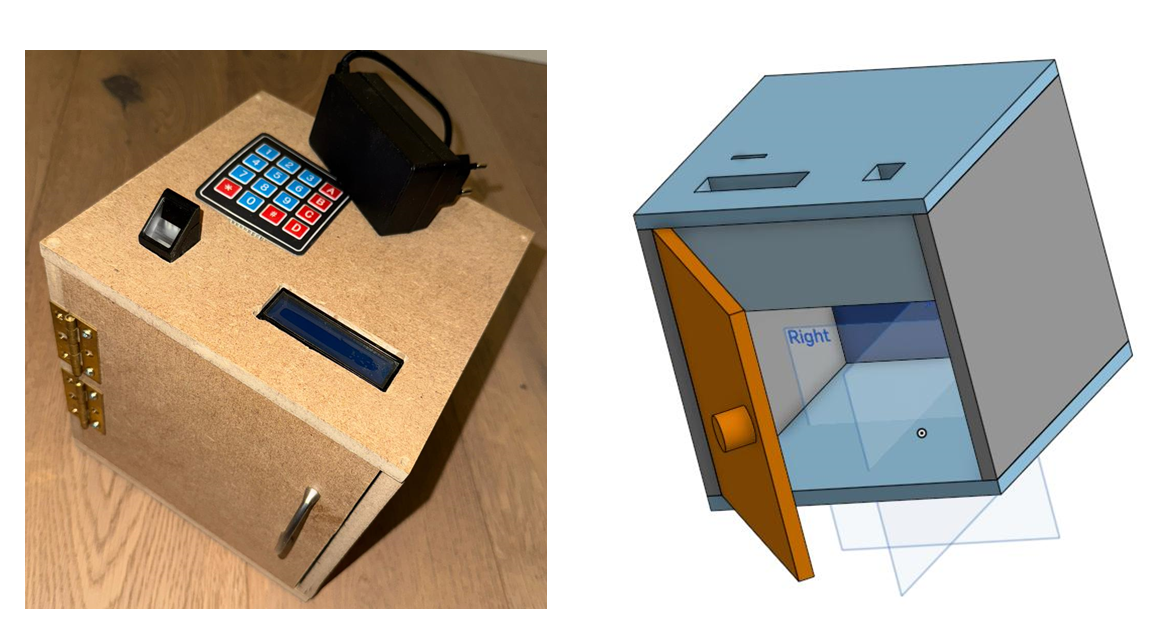
\includegraphics[width=\linewidth]{images/testpicture5.png}
    \captionsetup{hypcap=false}
    \captionof{figure}{Finished box on the left and 3D Design of the box on the right}
    \captionsetup{hypcap=true} 
\end{center}

    
\newpage
\section{Methods}
The development of the access control system involved a combination of hardware integration, software development, and custom physical design. This section outlines the key components used, their integration, and the construction process of the safe.

\subsection{Hardware Components}
The system utilized the following key hardware components:
\begin{itemize}
    \item \textbf{Arduino R4 Minima/R4 WIFI:} The central processing unit of the system, responsible for interfacing with all peripherals such as the fingerprint sensor, LCD display, and electromagnetic lock, while also handling communication via Wi-Fi when needed.
    \item \textbf{R307 Fingerprint Sensor:} Used for biometric authentication, capable of storing and verifying up to 1,000 fingerprints.
    \item \textbf{16x2 LCD Display:} Provides real-time feedback to the user, displaying messages such as "Access Granted" or "Place Finger..."
    \item \textbf{12V Electromagnetic Lock:} Secures the safe, controlled via a relay module to handle high-power requirements safely.
    \item \textbf{Wi-Fi Module:} Replaced the originally planned Real-Time Clock (RTC) to fetch time data from internet servers, ensuring accurate synchronization for time-based access control operations.
    \item \textbf{2-Channel Relay Module:} Facilitates power isolation between the Arduino and the 12V lock, ensuring safety and reliability.
    \item \textbf{RTC: } Initially intended for local timekeeping but was later substituted with an internet-based solution
    \item \textbf{Keypad 4x4:} Used for administrative functions, allowing authorized personnel to manage access permissions directly from the device.
\end{itemize}

\subsection{System Integration}
The design phase involved selecting the appropriate components that could be integrated into a cohesive system. We chose the Arduino as the microcontroller because of its versatility and support for multiple peripherals. The fingerprint sensor was selected for its high accuracy and reliability in biometric recognition. The LCD display was integrated to provide real-time feedback to users, and the keypad was incorporated for administrative control, allowing authorized personnel to manage access permissions directly from the device.

Each component was initially tested separately to verify its functionality. Once individual testing was successful, the components were integrated, and the system's overall functionality was tested. We developed a circuit diagram that outlined all connections, ensuring that each component was correctly interfaced with the Arduino. This careful planning helped mitigate potential issues during the integration phase.

    \begin{center}
         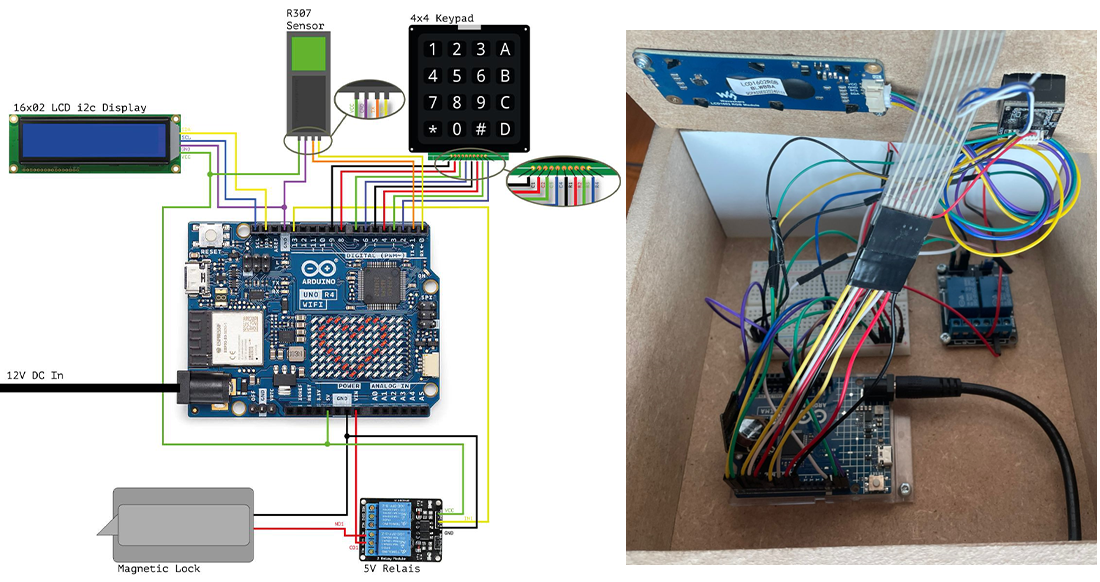
\includegraphics[width=1\linewidth]{images/Circuit-Box.png} 
         \captionsetup{hypcap=false}
         \captionof{figure}{ Design overview of complete circuit on the left and actual implementation on the right}
         \captionsetup{hypcap=true} 
    \end{center}


    

\subsection{Safe Construction}
The physical safe was designed using CAD software, creating a detailed blueprint with precise cutouts for the fingerprint sensor, keypad, and LCD display. The design also included a separate compartment to conceal the electronic components, ensuring both functionality and aesthetic appeal.

The CAD files were submitted to a hardware store for cutting the wooden components. These were then assembled manually, resulting in a functional safe with dual capabilities: it serves as a traditional storage safe and integrates the access control system.

\subsection{Software Development}
The software for the Arduino was written in C++, utilizing libraries tailored for the LCD, fingerprint sensor, and time synchronization. These include the \texttt{Waveshare LCD1602 RGB} library for display control, the \texttt{Adafruit Fingerprint} library for managing biometric data, and the \texttt{NTPClient} library for fetching real-time data via the Wi-Fi module.

The code structure prioritized modularity to allow independent testing and efficient debugging. Dedicated functions were implemented for adding or removing fingerprints, checking user access permissions, and managing time-based restrictions. Fingerprints are stored in the sensor's memory, with the ability to enroll new users by assigning them unique IDs or remove specific templates when necessary.

Time synchronization is handled by the Wi-Fi module, which retrieves accurate time data from online servers to enforce access restrictions, such as allowing entry only between 8:00 AM and 8:00 PM. Additionally, the master PIN system provides secure access to the menu for managing settings, ensuring administrative functions remain protected.

The software serves as the backbone of the system, seamlessly integrating all components and enabling reliable and user-friendly operation.

\newpage
\subsection{Challenges and Solutions}

Developing the fingerprint lock system with an LCD display involved a range of technical challenges that required systematic troubleshooting and innovative problem-solving approaches. These challenges encompassed hardware failures, integration difficulties, and unexpected setbacks that tested our problem-solving skills and adaptability.

\textbf{Voltage Misconfiguration:} Early in the integration phase, we encountered a major setback when the LCD and keypad were connected to a voltage higher than recommended. This oversight led to the malfunctioning of these components, necessitating their replacement. We implemented stricter checks for component specifications before integration, which helped prevent further hardware issues.

\textbf{Arduino Connectivity Issues:} Midway through the project, our Arduino board ceased to be recognized by any connected PC. This issue was critical as it halted our ability to upload new code and test modifications. After extensive troubleshooting, we concluded that the board was defective and replaced it. This incident underscored the importance of having backup components and reinforced our understanding of hardware management in complex projects.

\textbf{Real-Time Clock Integration:} Initially, the project planned to use a Real-Time Clock (RTC) for access control based on time constraints. However, we encountered persistent challenges in synchronizing it with the system accurately. As a solution, we transitioned to using the Arduino R4 WIFI, which includes a built-in Wi-Fi module, allowing us to fetch accurate time data from internet servers. This approach eliminated the need for an external RTC and improved system reliability.

\textbf{LCD Backlight Issue:} After replacing a faulty LCD display, we encountered an issue where the backlight did not illuminate at full brightness. Despite thoroughly checking the circuit and code configurations, the problem persisted. Ultimately, replacing the LCD with another new unit resolved the issue, highlighting the necessity of thorough quality checks and alternative troubleshooting methods.

The combination of hardware design, software development, and physical construction demonstrates the comprehensive effort involved in creating this system. The challenges encountered and the solutions implemented provided valuable learning experiences that contributed to the robustness and reliability of the final product.

\subsection{Obtained Results}

The final system met all our initial objectives, providing a secure, efficient, and user-friendly access control system. The fingerprint recognition was accurate, with no false positives in our tests. The administrative functionality allowed for easy management of user permissions, and the time-based access control operated flawlessly, restricting entry during off-hours as intended.

Furthermore, after incorporating the RTC module based on our professor's suggestion, we revised and enhanced the system by integrating an even more precise solution using the Wi-Fi module. This improvement significantly increased the accuracy of time synchronization and reduced maintenance efforts. The addition of the keypad further elevated the project's complexity, offering an additional layer of user input and security, leading to a more sophisticated final product than initially envisioned.

Through iterative improvements and thoughtful enhancements, we were able to refine the project beyond our initial expectations. We are highly satisfied with the visual appeal and practical usability of the final implementation.



\subsection{System Complexity and Achievements}
One of the project's most complex aspects was ensuring seamless integration and operation of the hardware components with the software. Achieving this required a deep understanding of each component's technical specifications and careful programming to handle various scenarios of user interaction and system response.

We are particularly proud of our development and integration of the administrative interface on the keypad and LCD. This interface allows system administrators to add or remove users efficiently, which is pivotal in environments that require high security with flexible access needs.

\newpage
\section{Closing Part}

\subsection{Division of Labor}
The project was a collaborative effort, with each team member contributing equally across various aspects of the project. In the initial stages, all three team members—Luca Fässler, Valerio Job, and Barthan Sivanantham—worked together to decide on the necessary hardware components to be used. Luca took on the responsibility of purchasing the selected components and ensuring their availability for the project.

The physical assembly of the system, including connecting all hardware components and troubleshooting integration issues, was carried out jointly by Luca and Valerio. Their hands-on collaboration ensured a smooth integration process and resolved any technical challenges that arose.

The software development phase saw equal contributions from all three members. Each played a crucial role in writing and refining the code to ensure the system's functionality met the desired specifications. Towards the later stages of the project, Barthan took on the responsibility of final revisions and optimization of the software. Throughout the project, Barthan documented all steps and changes made, ensuring a comprehensive record of the development process.

In terms of project reporting and presentation, Barthan initiated the creation of both the report and the presentation slides, laying the foundation for the final deliverables. However, all three team members collaborated on drafting, reviewing, and refining the content to ensure coherence and clarity.

\subsection{Critical Self-Assessment}
In retrospect, there were several areas where our project approach could have been improved. Firstly, the initial voltage misconfiguration that led to the malfunctioning of key components could have been avoided with a more meticulous initial review of the hardware specifications. This oversight highlighted the importance of thorough preparatory research and validation before proceeding with the integration of complex systems.

Secondly, while we managed to resolve the connectivity issues with the Arduino, having a backup strategy or additional testing hardware could have prevented the delays we experienced. Implementing routine backups of our development environment and code could also have mitigated the impact of hardware failures.

\subsection{Conclusions and Lessons Learned}
This project not only reinforced our technical skills in designing and implementing a biometric-based security system but also taught us valuable lessons in project management and teamwork. We learned the importance of clear communication and role allocation within the team, which were key to our project's success.

The challenges we encountered, such as hardware malfunctions and software bugs, provided us with firsthand experience in troubleshooting and problem-solving under pressure. These experiences have prepared us for similar challenges in future projects. Additionally, during this project, we overcame the problems with creative solutions, which in the end even improved the system. We also added more components, such as the keypad and a CAD-designed safe box, resulting in an even better and more user-friendly final product.

In conclusion, this project achieved its goals of developing a secure, efficient, and user-friendly access control system using biometric authentication. It has demonstrated the potential of integrating advanced technologies into practical applications, offering insights into both the complexities and rewards of working on interdisciplinary projects in the field of computer architecture.
\newpage
\section{Append}

\subsection{Disclaimer on Code Origin and Use of AI}
We confirm that the coding and design for the fingerprint-based security system were developed independently by our group members. The contents of this report and the underlying project it describes are entirely the result of our collaborative efforts. For the drafting of this report, we utilized ChatGPT solely to assist in refining the wording and improving the clarity of the narrative. We affirm that all technical content, results, and conclusions presented in this report are accurate and solely produced by us, reflecting our work on the project.

\subsection{Code Repository}
The project's source code, along with comprehensive documentation, is available on GitHub at the following link: 

\href{https://github.com/Lucafaessler/FingerprintLockProject.git}{https://github.com/Lucafaessler/FingerprintLockProject.git}

If additional access or specific details are required, please contact any of the three project team members.

\subsection{References}

\textbf{Component Vendors:}
\newline
\textbf{-Bastelgarage:} Most components used in the construction of the fingerprint-based security system were purchased from Bastelgarage (\href{https://www.bastelgarage.ch/}{www.bastelgarage.ch}) \\
\textbf{-Amazon:} Fingerprint Sensor R307S \\
\textbf{-Galaxus/Digitec:} Replacement Keypad and LCD Display, Replacement Arduino R4 WIFI\\
\textbf{-Jumbo:} Wood for the safe box, Hinge, Door Handle\\
\newline
\textbf{Libraries Used:}
\newline
\texttt{Wire.h}: Library for I2C communication.
\newline
\texttt{Waveshare\_LCD1602\_RGB.h}: Library for controlling I2C LCD displays.
\newline
\texttt{DIYables\_Keypad.h}: Library for managing matrix keypads
\newline
\texttt{Adafruit\_Fingerprint.h}: Library for interfacing with the Adafruit fingerprint sensor module
\newline
\texttt{WiFi.h}: Library for connecting to Wi-Fi networks
\newline
\texttt{WiFiUdp.h}: Library for sending and receiving UDP packets
\newline
\texttt{NTPClient.h}: Library for fetching time data from NTP servers
\newline
\texttt{SoftwareSerial.h}: Library for creating software serial ports
\newline
\newline
\textbf{Web References:}
\newline
No specific web references were used directly in the writing of this report. The descriptions and explanations are based on the collective knowledge and experience of the project group members.


\end{document}